\section{Software}
{\em Plumbing for the Arduino} was typeset using \LaTeX. Writing was carried out in either TextMate by Allan Odgaard or vi. Diagrams were produced using OmniGraffle Pro by the Omni Group, and screen captures were made using Snapz Pro by Ambrosia Software. 

The {\em completely awesome} circuit diagrams were made using Fritzing, an open source project that lets complete noobs design circuits visually, then see the same circuit as a schematic, and finally export that circuit as a PCB for etching by hand or automated manufacture. 

	\begin{figure}[h!]
	  \begin{center}
	    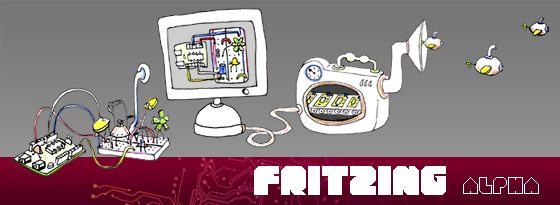
\includegraphics[width=0.9\linewidth]{images/20100110-frizing-splash-screen}
	    %\caption{A procedure call.}
	    %\label{pattern:ch1-proc-call}
	  \end{center}
	\end{figure}
	
Fritzing is truly a wonderful tool in progress; it was one of our discoveries while working on \plumbing. We had to to take a moment and gush its praises here---explore it, and discover the joy of circuit design.

\subsection{\occam and \plumbing}

\occam was originally designed under the guidance of David May, implemented by the fine people at \inmos, and shepherded by Professor Peter Welch at the University of Kent in Canterbury, England for the past 20 years (give or take). Many of the features that put the \mypi\xspace in \occam were implemented by Fred Barnes. 

The Transterpreter, which allows us to run \occam on tiny platforms like the Arduino, was originally designed and written by Christian Jacobsen and Matt Jadud, and extended and improved by Damian Dimmich, Carl Ritson, Adam Sampson, and Jon Simpson. The \url{concurrency.cc} board was designed by Omer Kilic. The \url{concurrency.cc} logo was designed by Geoffrey Long.

The \plumbing library was originally written by Christian Jacobsen, Matt Jadud, and Adam Sampson. Contributors since then include:

\begin{description}
	\item[Radu Creanga] Code for implementing PWM.
\end{description}

\newpage

\section{Images}
All images in this text were produced by the authors unless noted below. We have tried to use images placed in the Commons wherever possible.

The cover image was made available under a CC-BY license by Flickr user {\em macinate}:

\small{\url{http://www.flickr.com/photos/macinate/2191054677/}}

The T414 on page~\pageref{image:t414} was found on the Wikipedia under a CC-BY-SA-2.5 license:

\small{\url{http://en.wikipedia.org/wiki/File:IMST414B-G20S.JPG}}

The juggling LEGO figure on page \pageref{image:juggling} was made available by Flickr user {\em helico} under a CC-BY license:

\small{\url{http://www.flickr.com/photos/helico/404640681/}}

The image for ``waiting'' on page \pageref{medio:waiting} was made available by Flickr user {\em red twolips} under a CC-BY license:

\small{\url{http://www.flickr.com/photos/25182350@N03/2957915812/}}

\begin{comment}
	Juggling choices
	http://www.flickr.com/photos/teducation/2592566840/
	http://www.flickr.com/photos/sillylissy/2430488413/
	http://www.flickr.com/photos/helico/404640681/
	
	Waiting choices
	http://www.flickr.com/photos/myklroventine/3253953943/ (bus stop)
	http://www.flickr.com/photos/25182350@N03/2957915812/ (lady)
\end{comment}